\documentclass[a4paper,twoside, openright, 12pt, leqno]{article}
\usepackage[margin=0.5in]{geometry}
\usepackage{amsmath}
\usepackage{amsthm}                             % Proof environment
\usepackage{amssymb}
\usepackage{natbib}	
\usepackage{graphicx}

% New command \xbar to make bar wider
\newcommand*\xbar[1]{%
   \hbox{%
     \vbox{%
       \hrule height 0.5pt % The actual bar
       \kern0.3ex%         % Distance between bar and symbol
       \hbox{%
         \kern-0.28em%      % Shortening on the left side
         \ensuremath{#1}%
         \kern-0.05em%      % Shortening on the right side
       }%
     }%
   }%
} 


\title{Revision to the paper ``The threshold age of the lifetable entropy''}


\date{\today}
% Hint: \title{what ever}, \author{who care} and \date{when ever} could stand 
% before or after the \begin{document} command 
% BUT the \maketitle command MUST come AFTER the \begin{document} command! 
\begin{document}

\maketitle

\section*{Editor}
\textbf{Both reviewers made a point of requesting more on why e0 and the threshold age are so similar. I would recommend that the authors respond to this comment. this response could be  (1) the addition of  some additional analysis explaining the connection, (2) the addition of  a footnote or a few sentences in the text explaining why the connection is not so clear and is a topic for future investigations, or (3) a response letter with the final manuscript explaining why you chose not to address this. I suspect that it is possible to show that in the case where mortality is Gompertz that the threshold very nearly approximates e0. The derivation probably can be done using the logic of Vaupel (1986), in which a/b is assumed to be negligible in size. Then, the empirical correspondence with e0 comes from the fact that mortality is roughly Gompertzian.}
\linebreak

We thank the editor for his suggestions. We have addressed reviewers' concerns assuming a Gompertz hazard, as suggested by the editor. We included the following in the manuscript:

Assume the force of mortality follows a Gompertz distribution with hazard $\mu(x) = \alpha\,e^{\beta x}$, where $x\geq0$ denotes the age and $\alpha,\beta>0$ are parameters. The corresponding cumulative hazard is 
%%
$$
H(x) = \frac{\alpha}{\beta}\left( e^{\beta x} - 1 \right).
$$
%%
Following \cite{wrycza2014entropy}, the entropy of the lifetable can be expressed in terms of the Gompertz parameters as
$$
\xbar{H} = \frac{1}{\beta}\left( \frac{1}{e_o} - \alpha \right)\;,
$$
%%
where $e_o$ is the life expectancy at birth. Plugging in these two expressions into function $g(x)$ from Equation~(9) yields
\begin{equation}
g(x) = \frac{1}{\beta} \left( \alpha\,e^{\beta x} - \frac{1}{e_o} \right)+\,\xbar{H}(x)-1.
\label{eq.gx}
\end{equation}

From Equation~A1 in Proposition 1, the lifetable entropy conditioned on surviving to age $x$ can be expressed as
%%
$$
\xbar{H}(x)=\frac{e^\dagger(x)}{e(x)}=\frac{\int_x^\infty\,\ell(a)\,\big(H(a)-H(x)\big)\,da}{\int_x^\infty\ell(a)\,da}\;.
$$
%%
Using the above expressions in terms of the Gompertz parameters, it holds that
%
\begin{equation}
  \begin{split}
	\xbar{H}(x)
        & = \frac{\int_x^\infty \ell(a)\,\frac{\alpha}{\beta}\big(e^{\beta a}-e^{\beta x}\big)\,da}{\int_x^\infty\ell(a)\,da}=\frac{\int_x^\infty \ell(a)\,\alpha\,e^{\beta y}\,da}{\beta\int_x^\infty\ell(a)\,da} - \frac{\alpha}{\beta}\,e^{\beta x} 				\\
        & = \frac{\int_x^\infty\ell(a)\,\mu(a)\,da}{\beta\,e(x)\,\ell(x)} - \frac{\alpha}{\beta}\,e^{\beta x}=\frac{1}{\beta}\left(\frac{1}{e(x)}-\alpha\,e^{\beta x}\right)\;.
  \end{split}
  \label{eq.Hx}
\end{equation}
%
The last step in~\eqref{eq.Hx} uses the product $\ell(a)\,\mu(a)$ as the age-at-death distribution, which then implies that $\int_x^\infty \ell(a)\,\mu(a)\,da=\ell(x)$. Using~\eqref{eq.Hx}, $g(x)$ in~\eqref{eq.gx} reduces to

\begin{equation}
g(x) = \frac{1}{\beta}\left(\frac{1}{e(x)}-\frac{1}{e_o}\right)-1\;,
\label{eq.gx2}
\end{equation}
%
where $e(x)$ is the remaining life expectancy at age $x$. Equation~\eqref{eq.gx2} implies that the threshold age $a^H$ of the lifetable entropy $\,\xbar{H}$ under the Gompertz model occurs whenever
\begin{equation}
e(x) = \frac{1}{\beta+1\,/\,e_o}\;.
\label{eq.threshold}
\end{equation}

Following \citet{missov2013gompertz}, the remaining life expectancy at age $x$ in the Gompertz case can be approximated by
%
\begin{equation}
  e(x)\approx\frac{1}{\beta}\,e^{\alpha/\beta}\,\big(-\gamma-\ln(\alpha/\beta)-\beta x\big)\;,
  \label{eq:exapprox}
\end{equation}
%
where $\gamma\approx 0.57722$ is the Euler-Mascheroni constant. Using this result, the threshold age occurs whenever
%
\begin{equation*}
\begin{split}
e(x)	& \approx\frac{1}{\beta}\,e^{\alpha/\beta}\,\big(-\gamma-\ln(\alpha/\beta)-\beta x\big)=\frac{1}{\beta+1\,/\,e_o}			\\
& \Longleftrightarrow x=-\frac{e^{-\alpha/\beta}\,e_o}{\beta\,e_o+1}-\frac{1}{\beta}\,\big(\gamma+\ln(\alpha/\beta)\big)\;.
\end{split}
\end{equation*}

Replacing $e_o$ by the corresponding approximation from~\eqref{eq:exapprox}, we get
\begin{equation}
  \begin{split}
 	a^H & = -\frac{e^{-\alpha/\beta}\,e_o}{e^{\alpha/\beta}\left(-\gamma-\ln\left(\alpha\,/\,\beta\right)\right)+1}-\frac{1}{\beta}\,\big(\gamma+\ln(\alpha/\beta)\big)				\\
 	& = \frac{e^{-\alpha/\beta}\,e_o}{e^{\alpha/\beta}( \gamma+\ln\left(\alpha\,/\,\beta\right))-1}+\frac{e_o}{e^{\alpha/\beta}} \\
 	 	& = e_o \left(\frac{1}{e^{\alpha/\beta}}\right) \left(1  + \frac{1}{e^{\alpha/\beta}( \gamma+\ln\left(\alpha\,/\,\beta\right)) -1} \right)   \; \\
 	 	 	 	& = e_o \cdot \delta
  \end{split}
  \label{eq.x}
\end{equation}
%
which implies that the threshold age $a^H$ of the lifetable entropy $\,\xbar{H}$ for the Gompertz model is proportional to $e_o$ depending on $\delta$. From equation \eqref{eq.x}, the empirical correspondence between the threshold age and life expectancy at birth would come from $\delta$, which if it approximates one, it would  indicate that mortality in modern mortality schedules are roughly following a Gompertz model.
\linebreak

\begin{figure}[h!]
\caption{Factor value $\delta$ for threshold age under Gompertz distribution for French and Swedish women.}
\centering
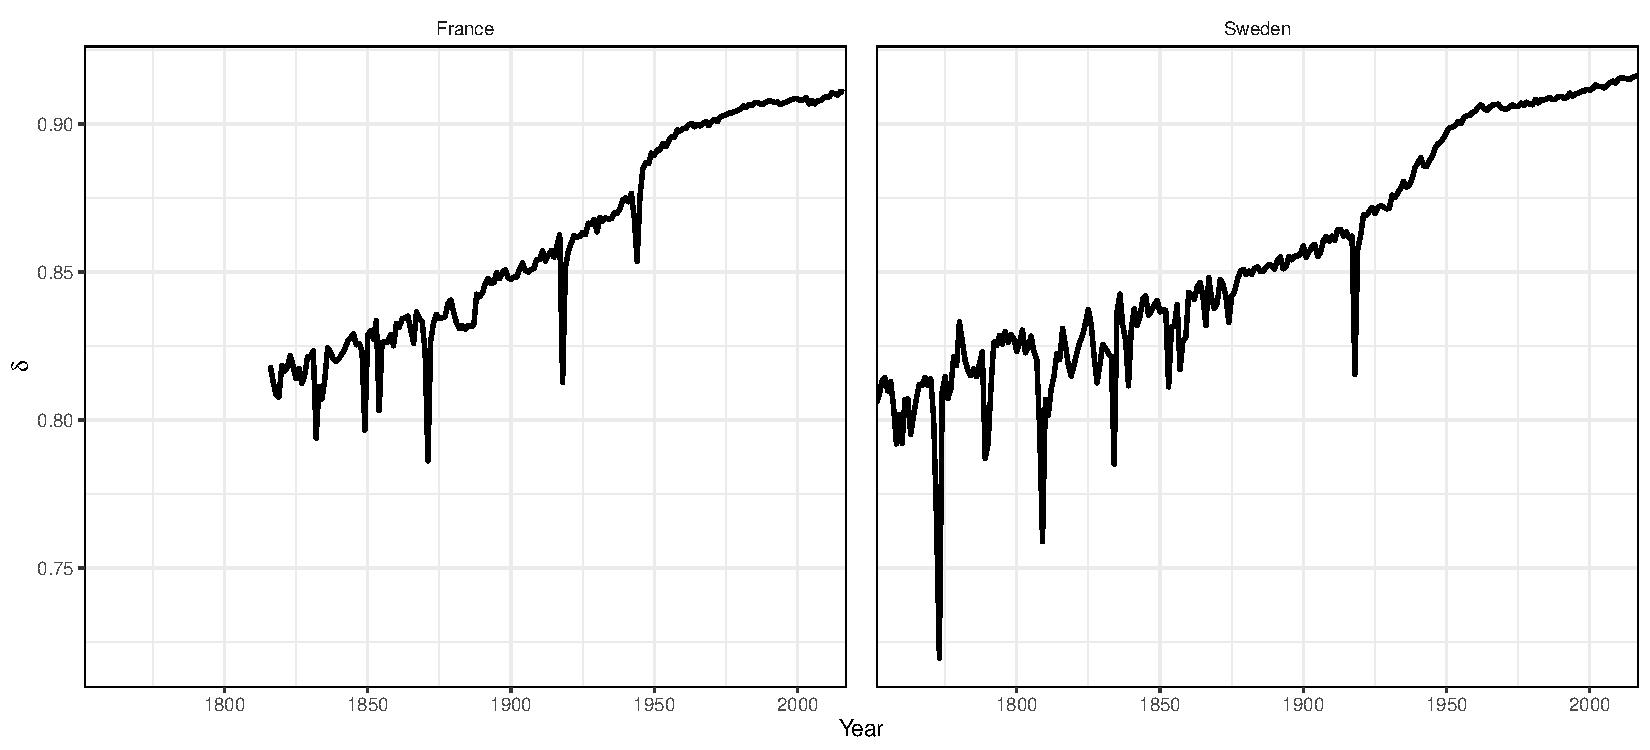
\includegraphics[scale=.5]{Figure_delta}
\end{figure}


%
%\noindent[VERSION 2: Lo que viene a continaucion es algo que he ido escribiendo en el proceso, aunque no lo pondria ya que creo que ha de primar la simplicidad. Pero como lo tengo hecho, pues por si lo quereis aprovechar]
%
%Following [ANYADIR Abramowitz and Stegun 1965??] \citet{missov2013gompertz} the remaining life expectancy at age $x$ in the Gompertz case is 
%%%
%$$
%e(x) = \frac{1}{\beta}\,e^{\alpha/\beta}\,E_1\left(\frac{\alpha}{\beta}\,e^{\beta x}\right),
%$$
%%%
%where $E_1(y)$ is the exponential integral 
%%%
%\begin{equation}
%  E_1(y) =\int_y^\infty\frac{e^{-t}}{t}\,dt=-\gamma-\ln(y)-\sum_{n=1}^\infty\frac{(-1)^n\, y^n}{n\cdot n!}\;, 
%  \label{eq:inteq}
%\end{equation}
%%%
%and $\gamma\approx 0.57722$ the Euler-Mascheroni constant. When $y=\alpha\,e^{\beta x}\,/\,\beta$ is close to 0, the summation on the right-hand side of~\eqref{eq:inteq} is negligible, and the remaining life expectancy of the Gompertz model can be approximated as
%$$
%  e(x)\approx\frac{1}{\beta}\,e^{\alpha/\beta}\,\left(-\gamma-\ln\left(\frac{\alpha}{\beta}\right)-\beta x\right)\;.
%$$
%
%Hence, the threshold age $a^H$ of the lifetable entropy $\,\xbar{H}$ under the Gompertz model occurs whenever
%%
%\begin{equation*}
%  \begin{split}
%	 e(x)	& \approx\frac{1}{\beta}\,e^{\alpha/\beta}\,\left(-\gamma-\ln\left(\frac{\alpha}{\beta}\right)-\beta x\right)=\frac{1}{\beta+1\,/\,e_o}			\\
%  	 & \Longleftrightarrow x=-\frac{e^{-\alpha/\beta}\,e_o}{\beta\,e_o+1}-\frac{1}{\beta}\left(\gamma+\ln\left(\frac{\alpha}{\beta}\right)\right)\;.
%  \end{split}
%\end{equation*}
%
%\noindent [END VERSION 2]
%\bigskip
%
%Then from \eqref{eq.threshold} the threshold age occurs when 
%%
%\begin{equation}
%\frac{1}{b} e^{a/b}\left[-\gamma - \ln\left(\frac{a}{b}\right) - bx - c \right] = \frac{1}{b+\frac{1}{e_o}},
%\label{eq.threshold2}
%\end{equation}
%%
%where $c = \sum_{n=1}^\infty \frac{(-1)^n (\frac{a}{b}e^bx)^n}{n \cdot n!}$ is the last term of the exponential integral. After some manipulation \eqref{eq.threshold2} yields
%
%%%
%$$
%-bx = e_o\left[ \frac{b}{e^{a/b}(e^{a/b}E_1(a/b)+1)} \right] + \gamma + \ln \left( \frac{a}{b} \right) + c.
%$$
%%%
%
%\noindent[PANCHO: Quiza me falla algo, pero aqui creo que no es correcto del todo: que C sea 0 no significa que $\gamma-\ln(a/b)$ lo sea]
%\bigskip
%
%To the extent that $c$ is close to 0, as suggested by \citet{missov2013gompertz}, then the threshold age $x$ from the above expression can be approximated by 
%%
%\begin{equation}
%  \begin{split}
%	x
%        & \approx e_o \left[\frac{1}{e^{a/b}}\left(1-\frac{1}{e^{a/b}(E_1(a/b)+1)} \right) \right] \\
%        & =  e_o \cdot \delta
%  \end{split}
%  \label{eq.x}
%\end{equation}
%%


\textbf{Reviewer 1’s point: What insight does the threshold age for entropy give above and beyond the threshold age for e dagger? Why would we calculate one over the other? also seems worth addressing in order to improve the motivation of the paper and attract more readers.
}

All lifespan variation indicators are different in the way they are constructed and their formal properties. In this sense, if one is interested in measuring relative inequality, then the lifetable entropy is a better indicator than $e^\dagger$, which is an indicator of absolute inequality. Another advantage of the lifetable entropy is that it captures the dimensionless shape of aging \citep{colchero2016emergence}, which is desirable when comparing age-at-death distributions of different species, for example. In this sense, if the lifetable entropy is used, the threshold age for $e^\dagger$ might be misleading regarding the effect of mortality changes, as we showed. This mismatch could lead to incorrect interpretation of some results. For example, in equation 10 in the manuscript, we are certain that if improvements happen at all ages, the early component is always negative (reducing the entropy) and the late component increases the entropy. This does not hold when the cut-off is derived with the threshold age of $e^\dagger$


\section*{Reviewer A}
\textbf{Main Strengths:
Overall, this is a clearly laid out and interesting paper. The mathematical relationships are clearly specified and easy to follow.} \\

\textbf{Main Weaknesses:
My only suggestions are for a bit more of a detailed discussion around the insight that the threshold age provides and around Figures 1 and 2. In particular: What insight does the threshold age for entropy give above and beyond the threshold age for e dagger? Why would we calculate one over the other? 
}
[Answered above and waiting for JAA and PV input]
\linebreak

\textbf{Looking at Figure 1, the natural question is “do we always expect the threshold age to be so close to e0?” Why or why not? Figure 2 somewhat answers this question with a “no” given the trends in historical periods, but this is not really discussed in the text. Why the convergence of the entropy threshold age and other measures (e0 and a dagger) over time? What is driving this? Given modern mortality conditions, do we always expect the threshold age to continue to be very close to life expectancy? Or is it possible it will diverge again with improvements at older ages?} 
[Answered above and waiting for JAA and PV input]





\section*{Reviewer B}
\textbf{Main Strengths:
The paper presents interesting results related to an important measure for mortality studies, the Keyfitz entropy. The derivations are clear and provide useful and elegant results. These are certainly of interest to readers of the special collection on "Formal Relationships."}\\

\textbf{Main Weaknesses:
The point where the article could be improved is the "Applications" chapter. The authors could discuss in more details the interpretation of the threshold age for Keyfitz's, compared to e0 and the threshold age for e-dagger, as well as the implications of the findings of the paper for understanding mortality change and inequality of lifespans.} [Answered above and waiting for JAA and PV input]\\

\textbf{Figure 2 presents intriguing results, but are not clearly interpreted in the paper. A few examples of topics that would be interest to discuss are: what are the features of mortality curve that make e0 and the threshold age for Keyfitz's entropy to converge?; and why were them so different for early years?; why is the threshold age for Keyfitz's entropy smoother than the other measures, even in periods of great mortality variation?} [Answered above and waiting for JAA and PV input]\\

Recommendations to Author:
In addition to the recommendation to expanding the interpretation of the results, there are a few minor suggestions:\\
On page 1, line 7, l(a) and l(x) are missing the t index.\\
On page 1, line 14, complement the sentence “remaining life expectancy at age a” with “at time t”.\\
On page 9, there is a typo in “Not the similarity”. \\
Review the last sentence of the conclusion, item (2). It doesn’t explain precisely what the threshold is about.

\textbf{We thank the reviewer for the careful read of our paper. Following his/her advice we have made all the changes suggested.}

\bibliographystyle{dinat}
\bibliography{Bib_FormalDemo}

\end{document}
